\chapter{Framework}
\label{ch:Framework}

In this chapter the description of the framework development is given. In first sections the conceptual model and the architecture of the solution are discussed. Further sections provide the details of the solution implementation.

\section{Framework Conceptual Model}

\section{Framework Architecture}

\section{Framework Implementation}

\subsection{Input Data Description (Nature of Data)}

According to the research done by the US Department of Transportation based on data of Fatality Analysis Reporting System (FARS) and National Automotive Sampling System, nearly 40 percents of all the reported in 2008 year crashes were road intersection related \cite{inproceedings:10_cfi}. Consequently, cross-road transport activity analysis is significantly important nowadays in context of safety, and identifying unsafe vehicular trajectories, which violate traffic rules, may be one of the steps towards improving the statistics.

In the presented work video from enforcement cameras is used for training and testing. Test videos are captured using the Intellectual Transportation Systems implemented on four different Kazan crossroads:
\begin{enumerate}
	\item An intersection of Pravo-Bulachnaya and Puschkina streets (Figure \ref{fig:is_1}).
	\item An intersection of Nesmelova and Kirovskaya Damba streets (Figure \ref{fig:is_2}).
	\item An intersection of Moskovskaya and Galiaskara Kamala streets (Figure \ref{fig:is_3}).
	\item An intersection of Moskovskaya and Parizhskoy Kommunyi streets (Figure \ref{fig:is_4}).
\end{enumerate}

Each crossroad corresponds to a 4-way intersection and is equipped with a single monitoring camera. Sample pictures from surveillance cameras are given below on Figures \ref{fig:is_1} -- \ref{fig:is_4}.
\begin{figure}[!htb]
	\centering{}
	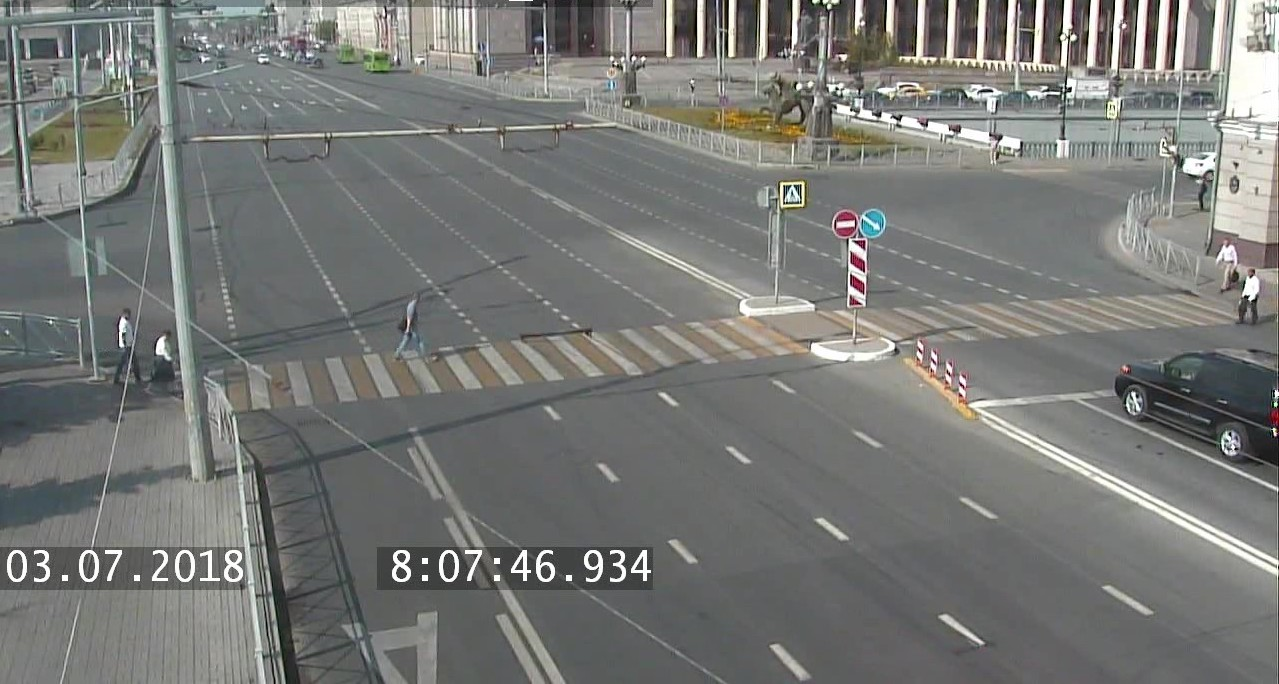
\includegraphics[width=0.8\textwidth]{images/is-1.jpg}
	\caption{Pravo-Bulachnaya / Puschkina intersection}
	\label{fig:is_1}
\end{figure}
\begin{figure}[!htb]
	\centering{}
	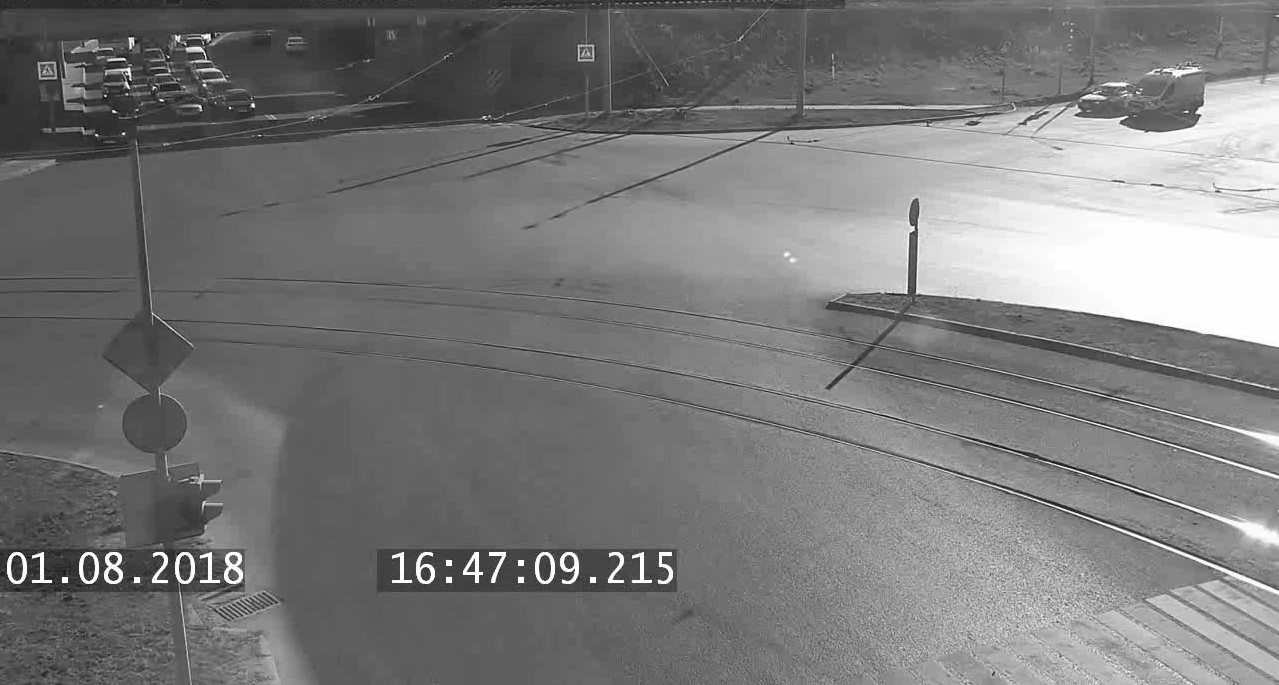
\includegraphics[width=0.8\textwidth]{images/is-2.jpg}
	\caption{Nesmelova / Kirovskaya Damba intersection}
	\label{fig:is_2}
\end{figure}
\begin{figure}[!htb]
	\centering{}
	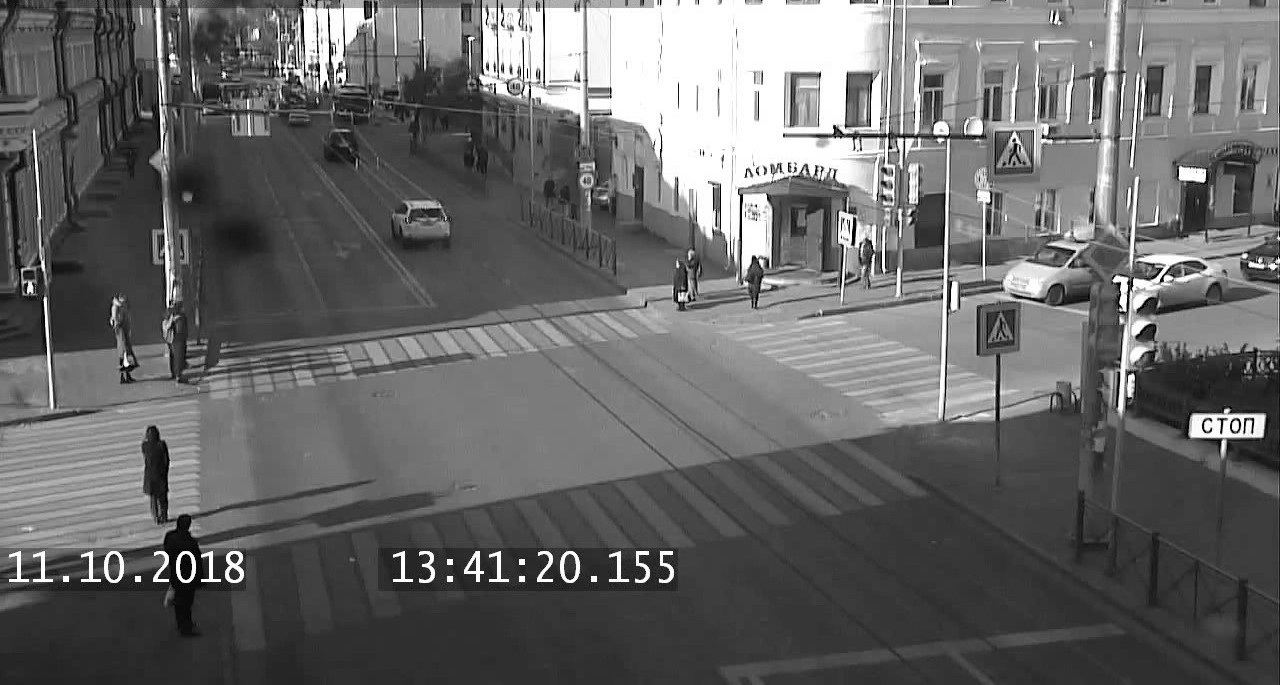
\includegraphics[width=0.8\textwidth]{images/is-3.jpg}	\caption{Moskovskaya / Galiaskara Kamala intersection}
	\label{fig:is_3}
\end{figure}
\begin{figure}[!htb]
	\centering{}
	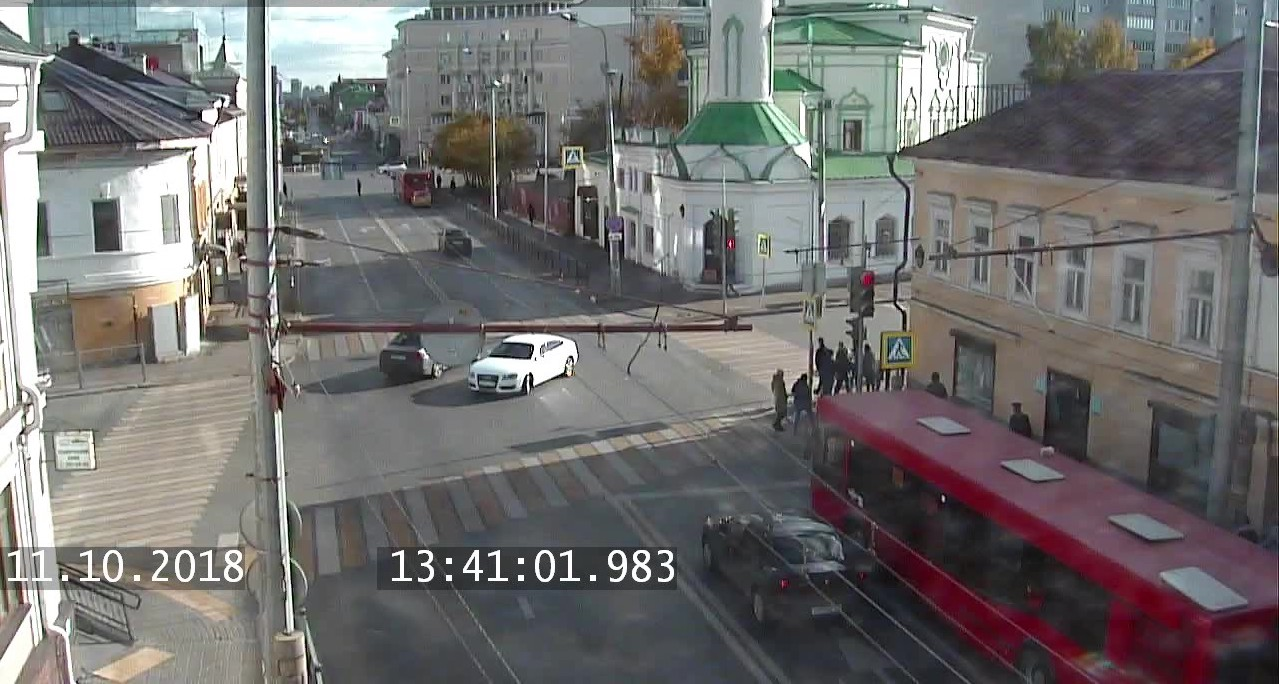
\includegraphics[width=0.8\textwidth]{images/is-4.jpg}
	\caption{Moskovskaya / Parizhskoy Kommunyi intersection}
	\label{fig:is_4}
\end{figure}

Input data files contain 624, 211, 231, 237 vehicular trajectories for the each of the aforementioned intersections respectively.

By a trajectory anomaly we understand vehicle trajectories through the crossroad, which remarkably differ from majority of common, known trajectories. For example, if no turning to the right from the left line is allowed, such a behavior will be unknown and such a trajectory must be considered as an anomaly.

\begin{figure}[!htb]
	\centering{}
	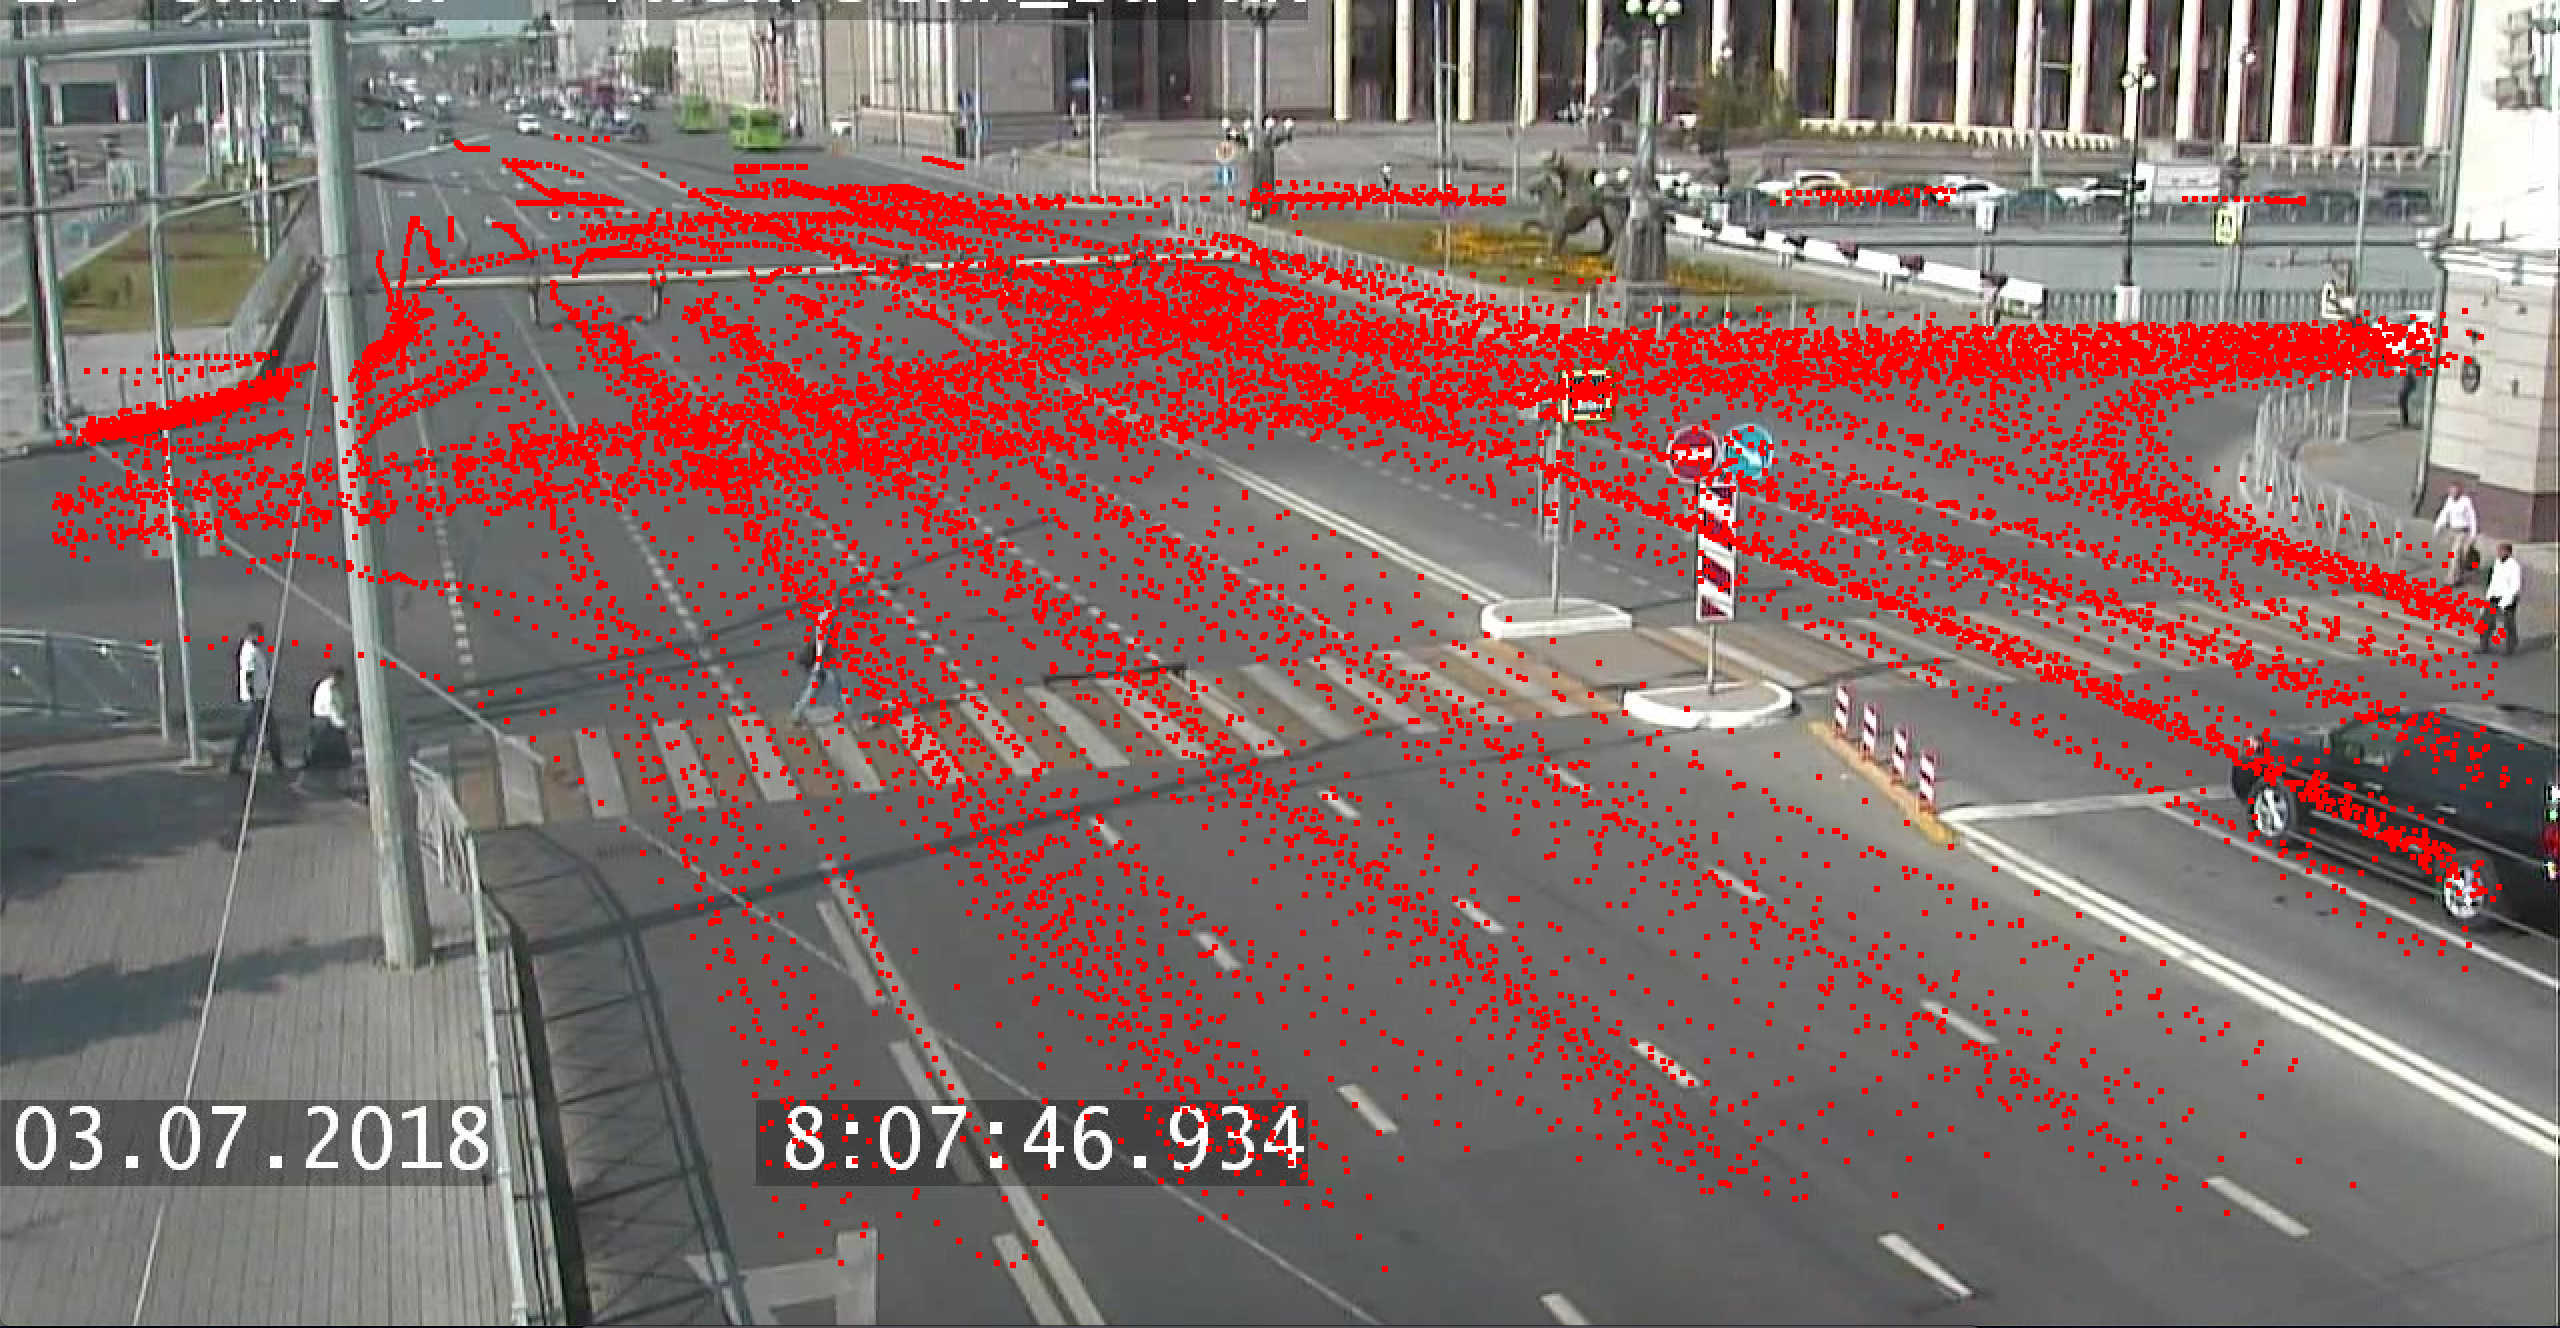
\includegraphics[width=0.8\textwidth]{images/tr-p.png}
	\caption{Output of a tracking system for video the first intersection}
	\label{fig:tr_p}
\end{figure}

\subsubsection{Input data file structure}
Tracking system, as it was described before, handles video from enforcement cameras and prepare it for further analysis: converts video stream into a set of vectors with tracking points on images (Figure \ref{fig:tr_p}).

Input data files have the following structure:
\begin{equation} \label{eq:input_str}
	[[[(x_1^1, y_1^1), ..., (x_1^n, y_1^n)], [t_1, ... t_n]], [[(x_2^1, y_2^1), ..., (x_2^m, y_2^m)], [t_1, ... t_m]], ...]
\end{equation}

As it can be seen from the input data file structure, each trajectory is represented by a two-element array, where first array stores coordinates as an array of two-tuples $(x_i^j, y_i^j)$ and second array contains timestamps for each spatial point in the corresponding order $(t_i)$. The extracted $x$- and $y$-coordinates correspond to pixels on input images. In Formula \ref{eq:input_str} the lower index of the spatial coordinates indicates the ordering number of a trajectory, while the upper index indicates the ordering number of a tracking point. The outer array refers to the array of trajectories.


\subsection{Input Data Processing}
Since chosen algorithm requires trajectories in a form of multi-dimensional vectors, the initial input data needs to be converted into the required form. For that reason, a custom parser was implemented. It takes a ‘txt’ file with trajectories as an input and as a result it returns a list of Trajectory objects. Trajectory object consists of a number of TrajectoryPoint objects with following information: \textit{x}-coordinate, \textit{y}-coordinate, time \textit{t}. The source code of the parsing method is presented in the Listing in Appendix chapter.